

\begin{frame}[ctb!]
  \frametitle{Extensions : Fracturation}
    \begin{minipage}{0.49\textwidth}
      \begin{figure}[h!]
        \includegraphics[width=\textwidth]{./images/fracturesAB.eps}
        \label{fig:fracturesAB}
      \end{figure}
    \end{minipage}
    \hspace{.01cm}
    \begin{minipage}{0.49\textwidth}
      \begin{figure}[h!]
        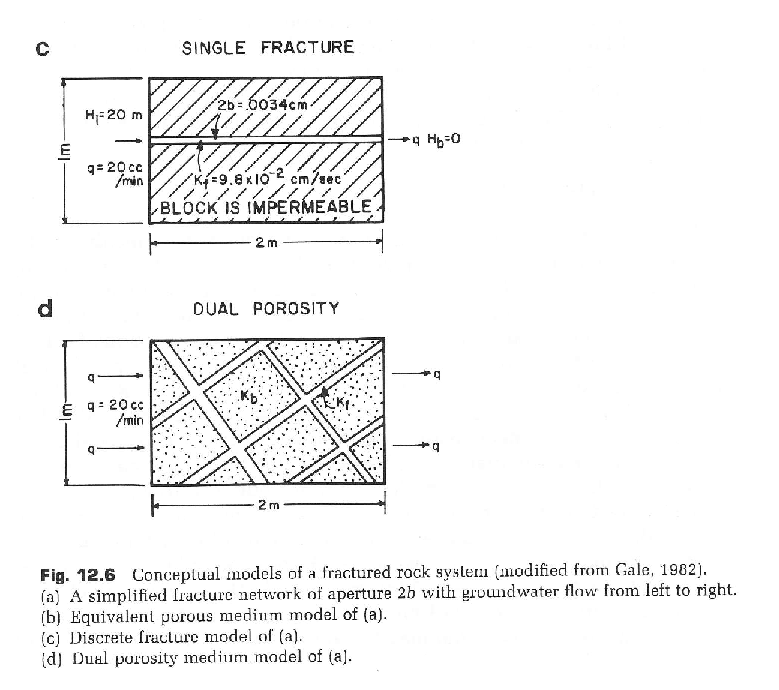
\includegraphics[width=\textwidth]{./images/fracturesCD.eps}
        \label{fig:fracturesCD}
      \end{figure}
    \end{minipage}

  A dual continuum model will be implemented to more accurately represent 
  fractured host media such as granite \cite{anderson_applied_1992}.
\end{frame}


\begin{frame}[ctb!]
  \frametitle{Extensions : Sorption}
  \begin{figure}[h!]
      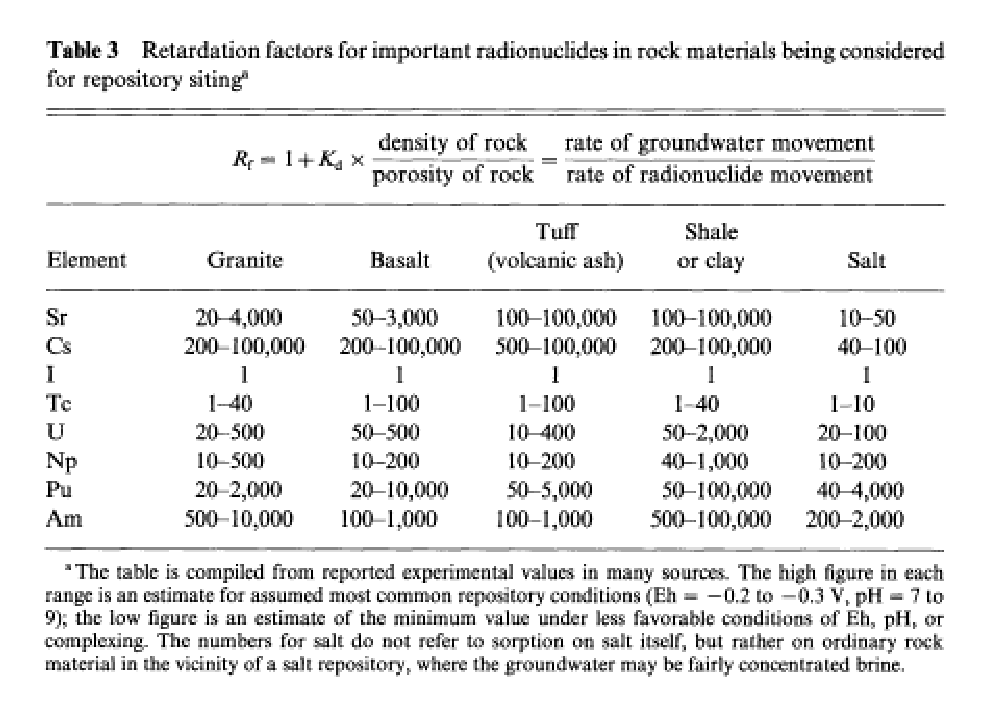
\includegraphics[height=.75\textheight]{./images/sorptionKrauskopf.eps}
    \caption{Sorption will be modeled using retardation factors in the mixed 
    cell models \cite{krauskopf_geology_1988}.}
    \label{fig:sorptionKrauskopf}
  \end{figure}
\end{frame}


\begin{frame}[ctb!]
  \frametitle{Extensions : Coalescence}
  Salt and clay exhibit coalescent behavior under heat. This decreases both the 
  buffer volume and the porosity in the near field.
  \begin{figure}[h!]
    \begin{center}
      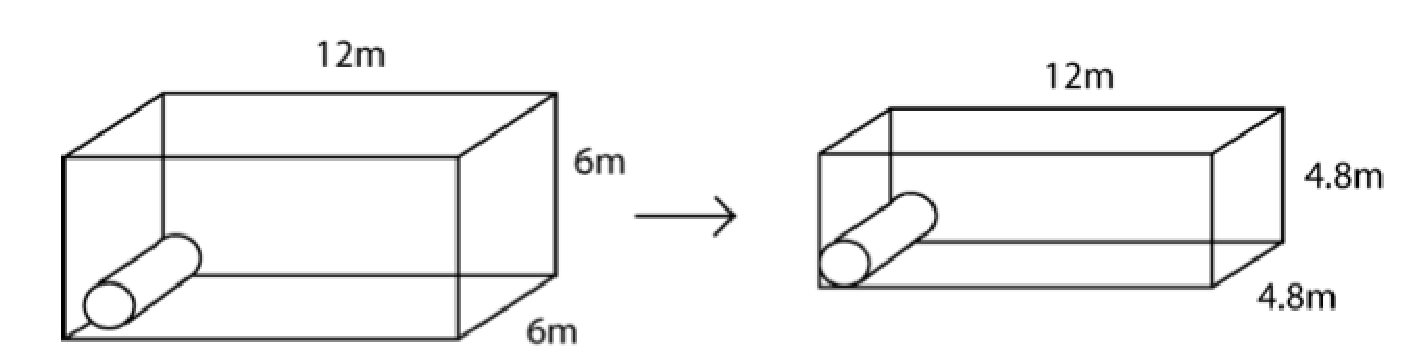
\includegraphics[width=\textwidth]{./images/saltAlcoveGPAM.eps}
    \end{center}
    \caption{The UFD salt Generic Disposal System Model incorporates salt 
    coalescence by modeling an alcove which decreases in size 
    \cite{clayton_generic_2011}.}
    \label{fig:saltAlcoveGPAM}
  \end{figure}
\end{frame}

